\section{PROCEDIMIENTO} 
\begin{itemize}
	\item Paso 1: Abrir Visual Studio, Crear una solucion Web  [Aplicacion web ASP.NET(.NET Framework)]\\
		\begin{center}
		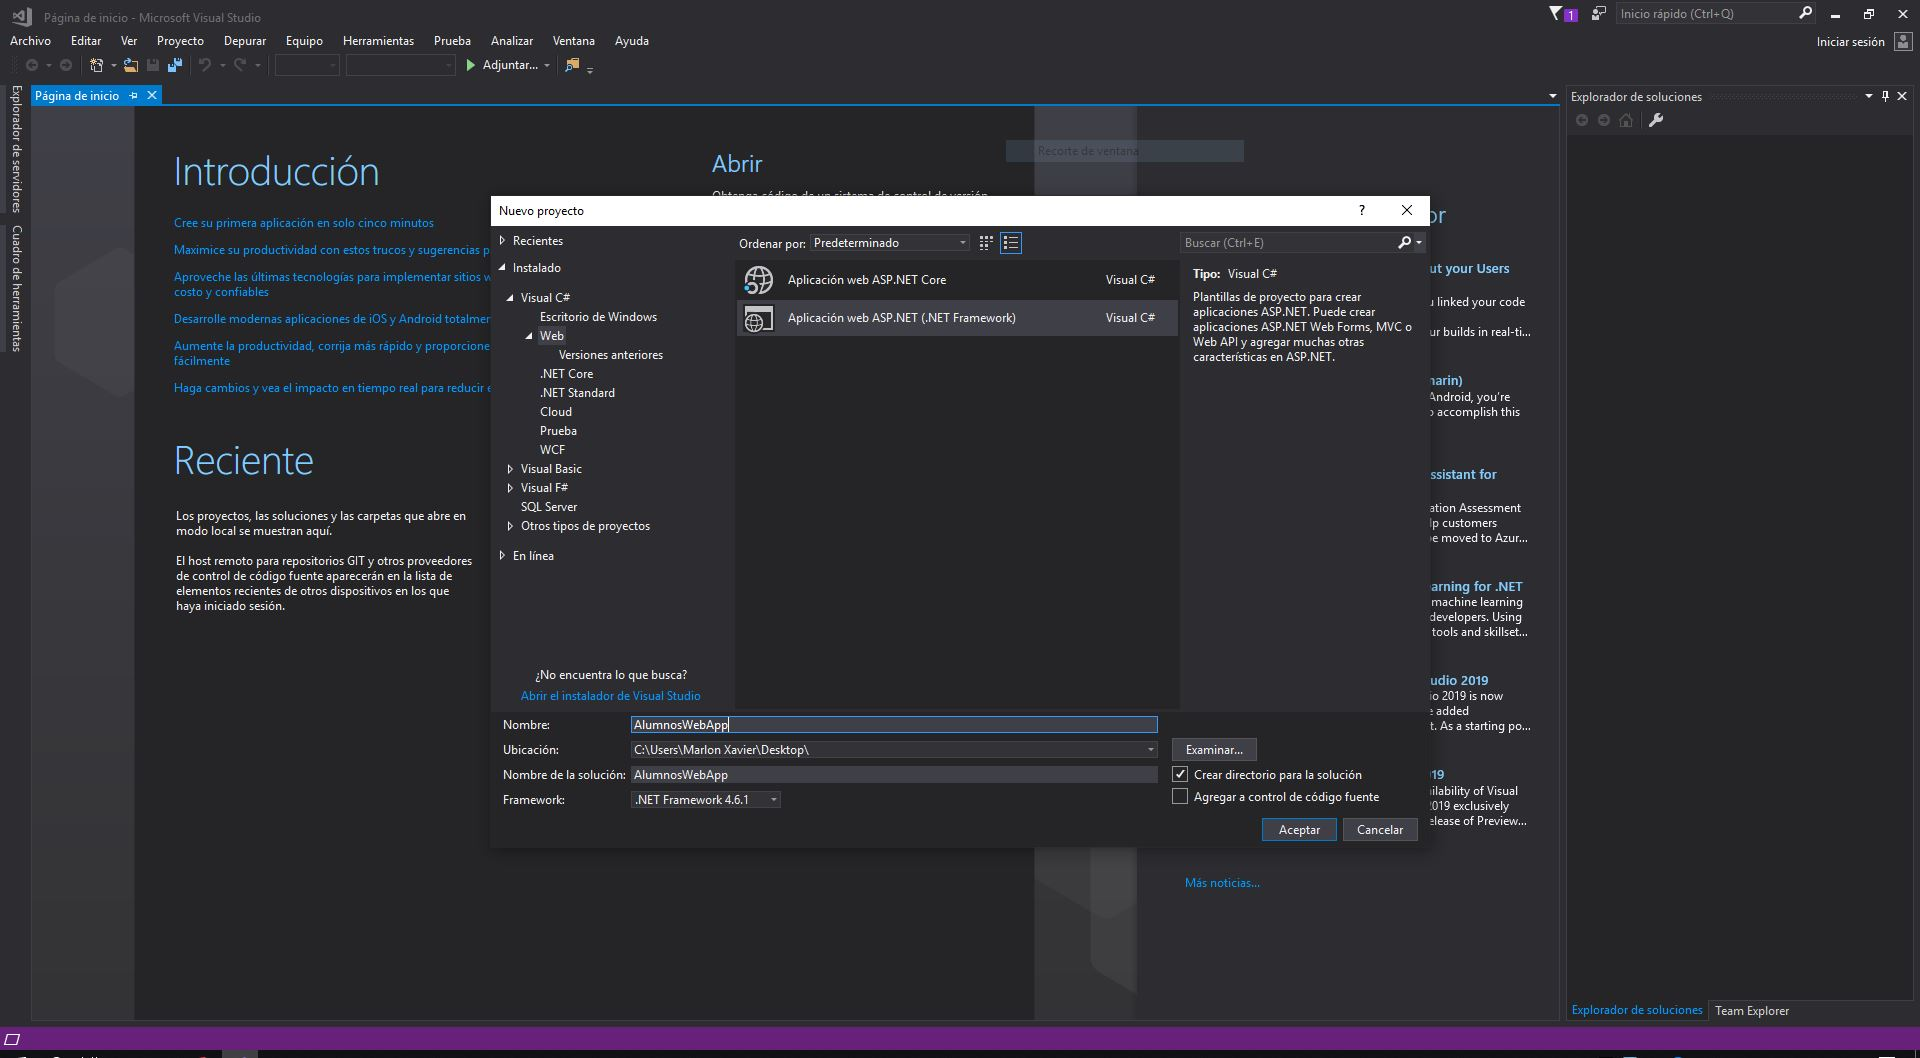
\includegraphics[width=15cm]{./Imagenes/Captura1}
		\end{center}
	\item Paso 2: Seleccionar la plantilla (Web API) con las opciones (MVC  y API web) marcadas\\
	\begin{center}
		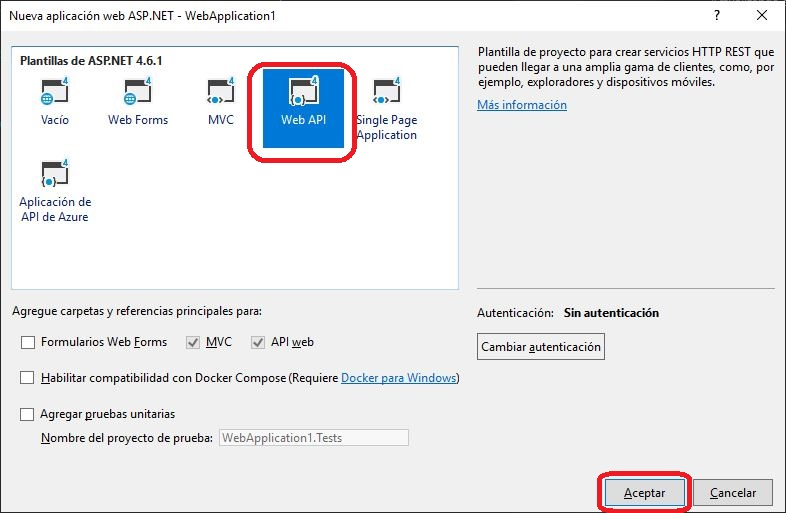
\includegraphics[width=15cm]{./Imagenes/Captura2}
		\end{center}
	\item Paso 3: Una vez creada la solución, dentro de la carpeta (Models)\\ Agregar 3 clases llamadas (Alumno, Tarea, TareaAlumno)\\
	\begin{center}
		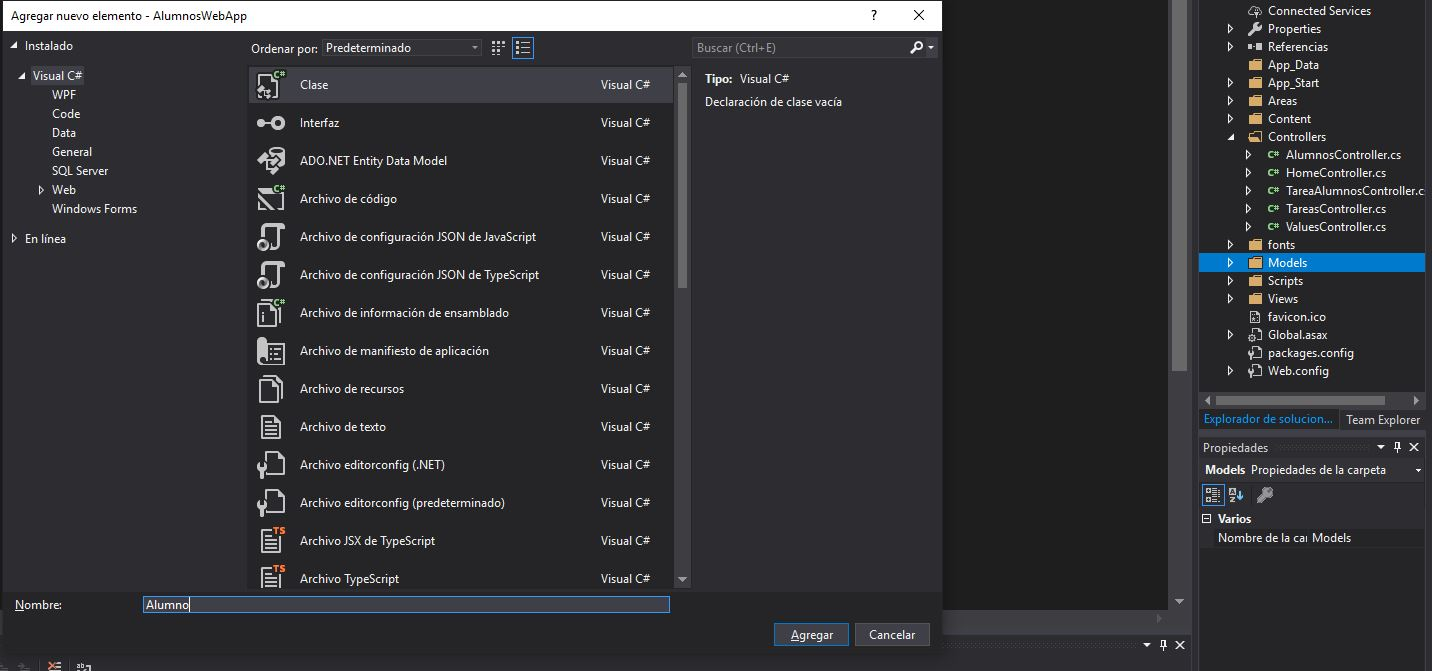
\includegraphics[width=15cm]{./Imagenes/Captura3}
		\end{center}
	\item Paso 4:Dentro de cada clase ingresar el codigo correspondiente a la siguiente imagen\\ (tener en cuenta agregar en la clase TareaAlumno:\\
	using System.Component.Model.DataAnnotations;\\
	using System.Component.Model.DataAnnotations.Schema;)\\
	\begin{center}
		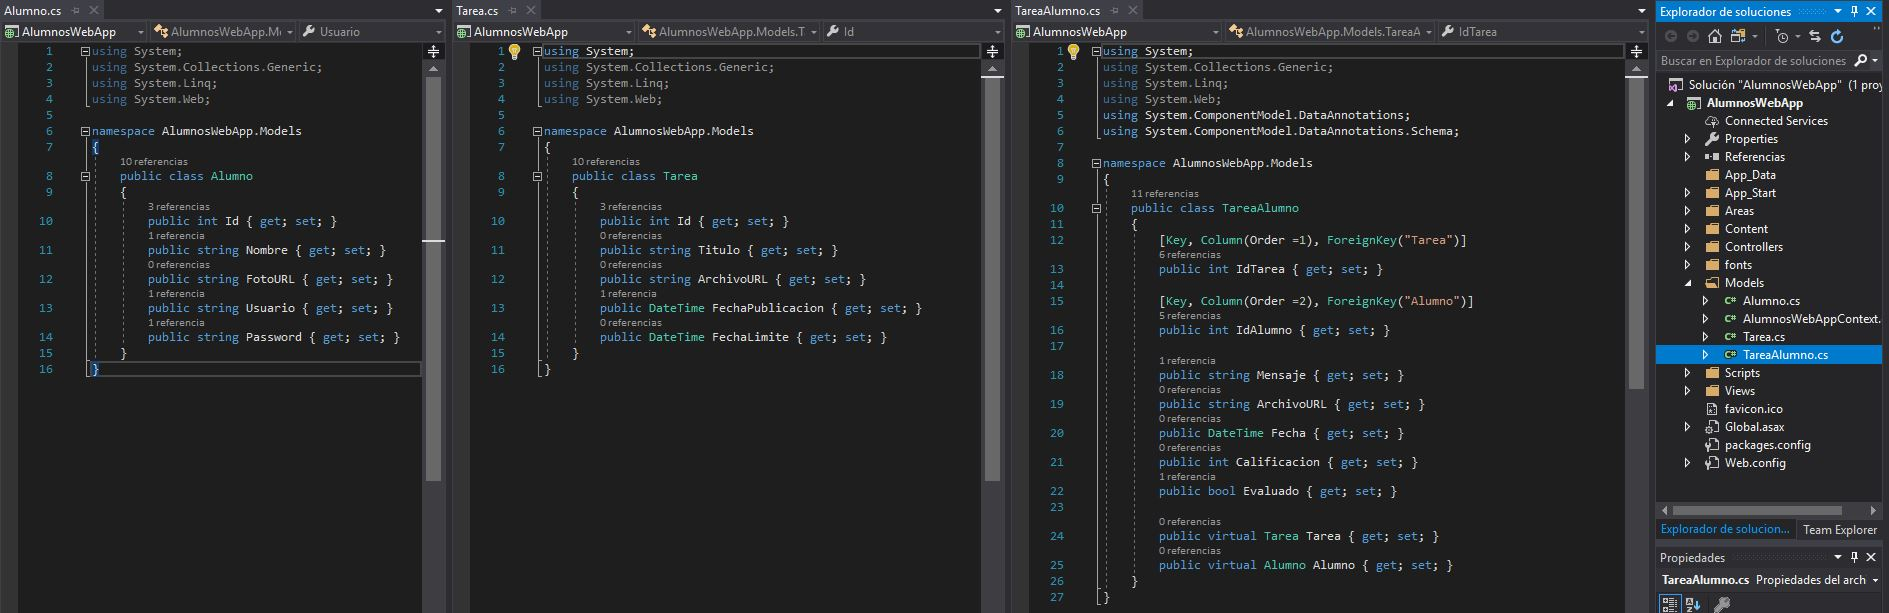
\includegraphics[width=15cm]{./Imagenes/Captura4}
		\end{center}
		\newpage
	\item Paso 5: Luego de terminar con las clases en Models, Pulsamos click derecho en la raiz de la solucion y por seguridad seleccionar las 3 primeras opciones(Para evitar errores al continuar con los siguientes pasos)\\
	\begin{center}
		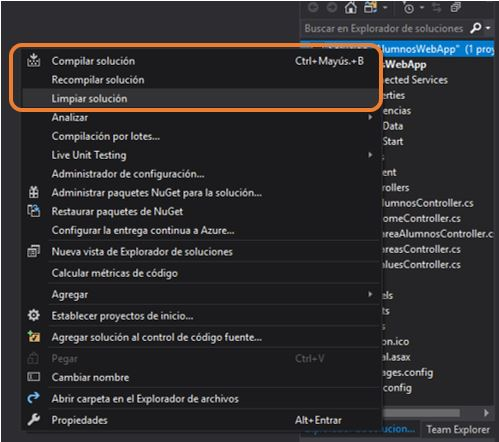
\includegraphics[width=15cm]{./Imagenes/Captura6}
	\end{center}
	\newpage
	\item Paso 6: Ahora hay que dirigirnos a la carpeta Controllers\\ 
	En la carpeta le damos a Agregar - Controlador\\
	\begin{center}
		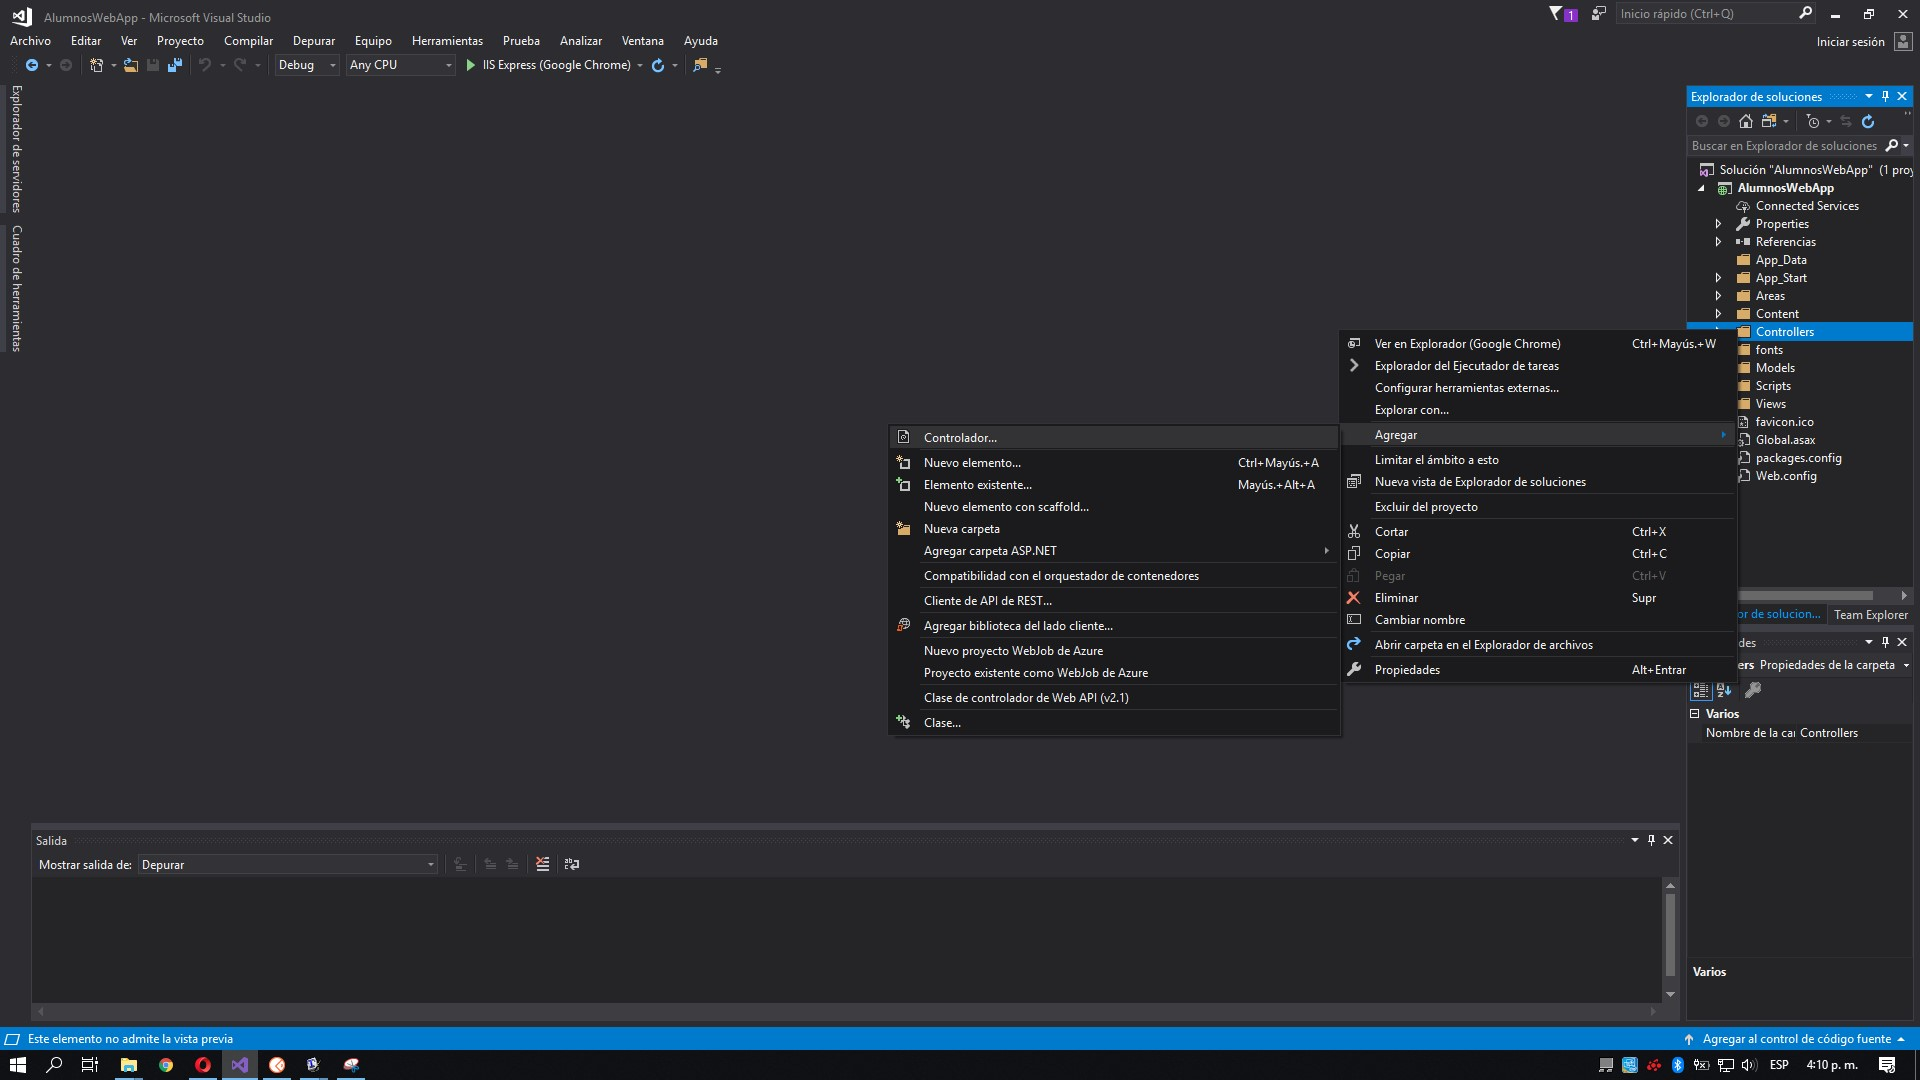
\includegraphics[width=15cm]{./Imagenes/Captura5}
	\end{center}
	\item Paso 7: En la ventana que nos aparece, Seleccionar la Opcion\\
	Controlador de Web API 2 con acciones que usan Entity Framework\\
	\begin{center}
		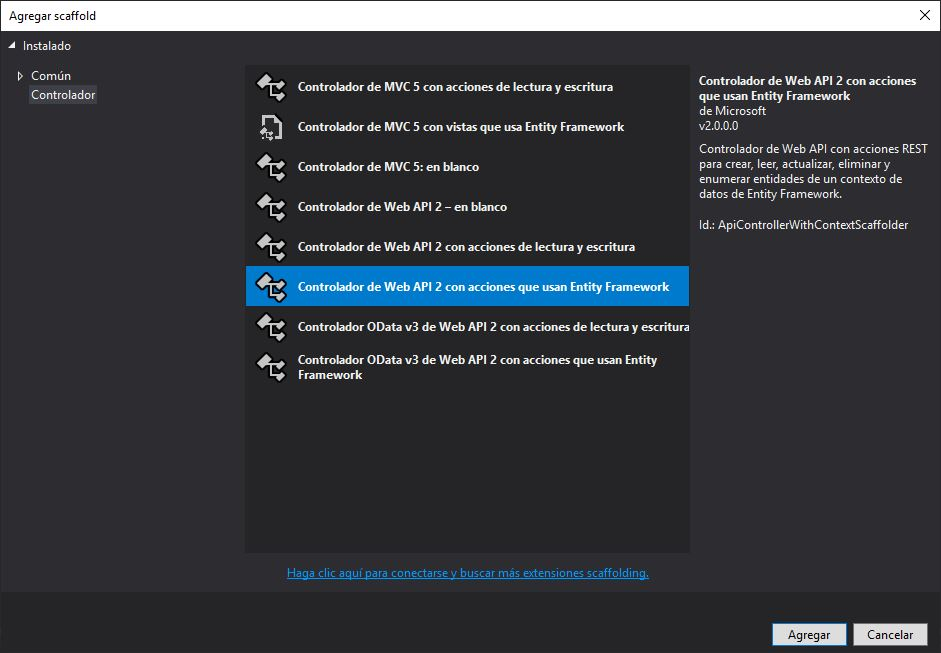
\includegraphics[width=15cm]{./Imagenes/Captura7}
	\end{center}
	\item Paso 8: Aparecerá una ventana para Agregar Controllador\\
	hacer lo mostrado en la imagen\\
	\begin{center}
		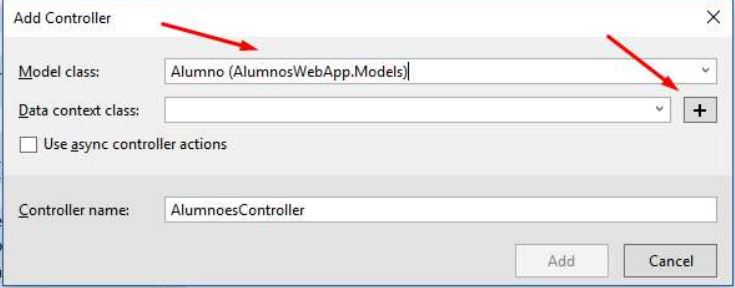
\includegraphics[width=15cm]{./Imagenes/Captura8}
	\end{center}
	\item Paso 9: Por defecto nos genera el nombre para el Nuevo Contexto de Datos, pulsamos Agregar o Add\\
	\begin{center}
		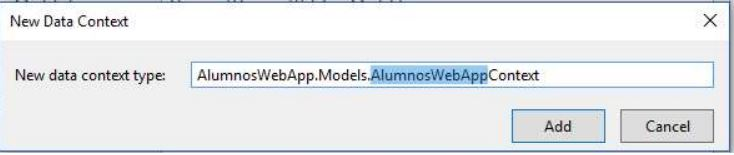
\includegraphics[width=15cm]{./Imagenes/Captura9}
	\end{center}
	\item Paso 10: Cambiamos el Nombre del Controlador de (AlumnoesController  a  AlumnosController) y Pulsamos Add\\
	\begin{center}
		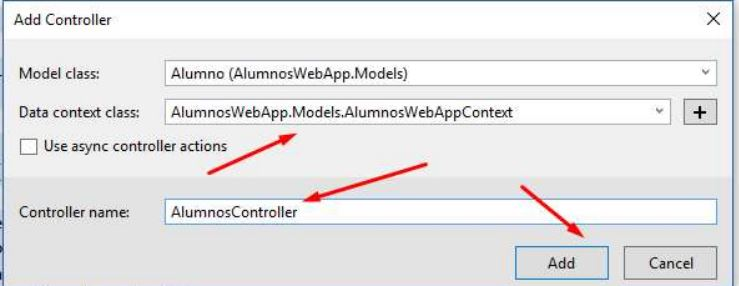
\includegraphics[width=15cm]{./Imagenes/Captura10}
	\end{center}
	\newpage
	\item Paso 11: Una vez creado el controlador AlumnosController\\
	Modificamos y agregamos condigo dentro de //GET: api/Alumnos\\
	\begin{center}
		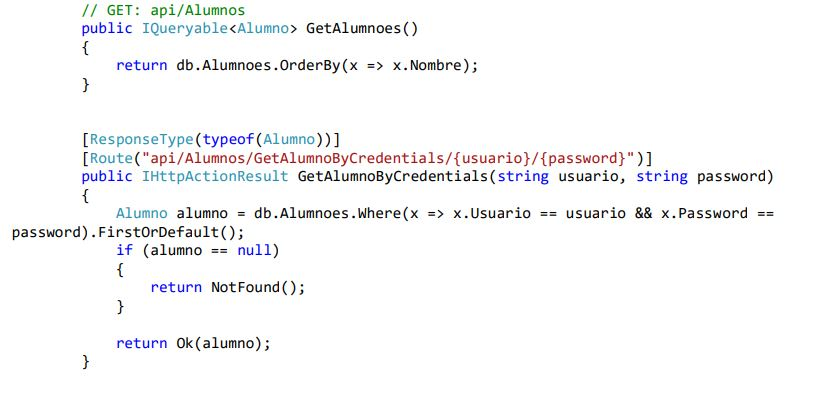
\includegraphics[width=15cm]{./Imagenes/Captura11}
	\end{center}
	\item Paso 12: Al igual que el anterior controllador, Agregamos un controlador nuevo llamado TareasController\\
	\begin{center}
		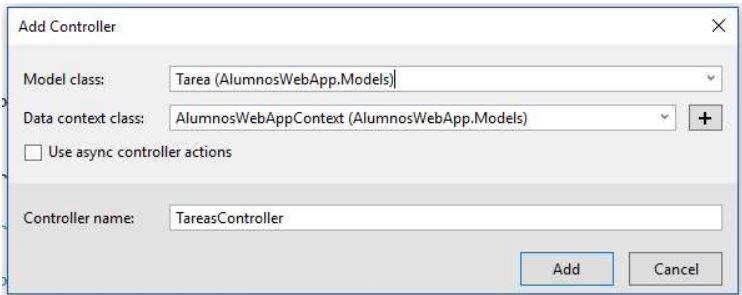
\includegraphics[width=15cm]{./Imagenes/Captura12}
	\end{center}
	\item Paso 13: Ahora dentro del controlador TareasController solo modificamos en // GET: api:Tareas  la linea (return db.Tareas)\\
	\begin{center}
		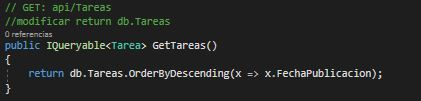
\includegraphics[width=15cm]{./Imagenes/Captura13}
	\end{center}
	\item Paso 14: Agregamos un ultimo controlador, Este se llamara TareaAlumnosController\\
	\begin{center}
		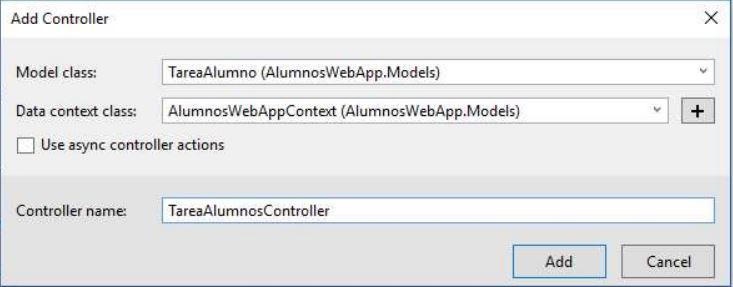
\includegraphics[width=15cm]{./Imagenes/Captura14}
	\end{center}
	\newpage
	\item Paso 15: Reemplazamos todo el código con las siguientes imagenes\\
	\begin{center}
		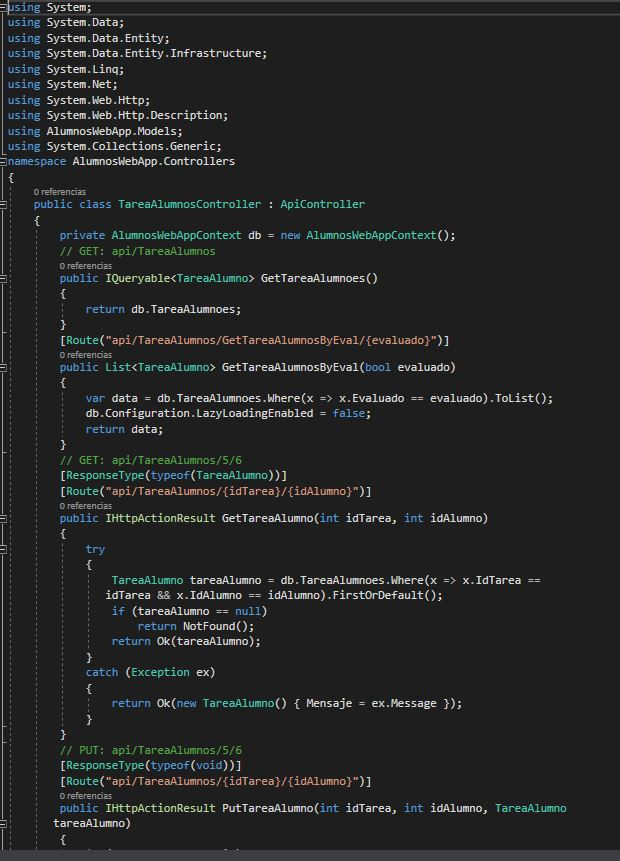
\includegraphics[width=15cm]{./Imagenes/Captura15}
		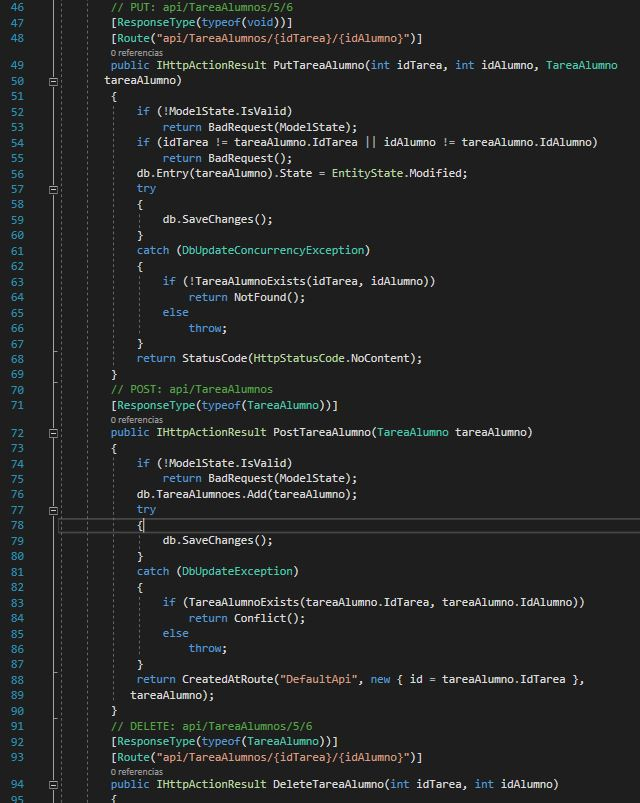
\includegraphics[width=15cm]{./Imagenes/Captura16}
		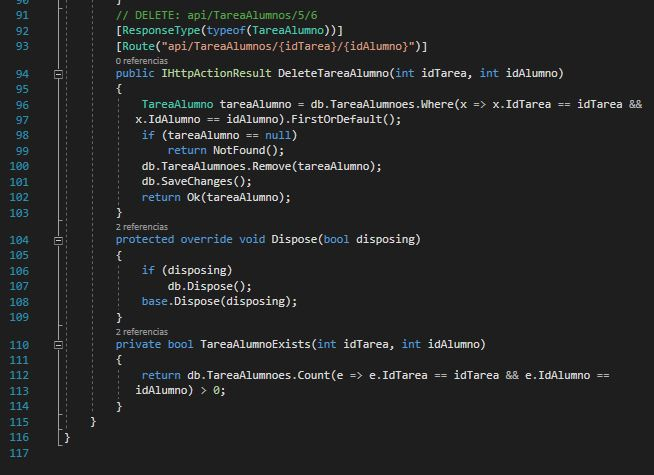
\includegraphics[width=15cm]{./Imagenes/Captura17}
	\end{center}
	\item Paso 16: Una vez terminado, Ejecutamos la solucion\\
	\begin{center}
		
\includegraphics[width=15cm]{./Imagenes/Captura18}
	\end{center}
	\item Paso 17: Se abrirá un navegador (en este caso chrome) y debemos pulsar la opcion API\\
	\begin{center}
		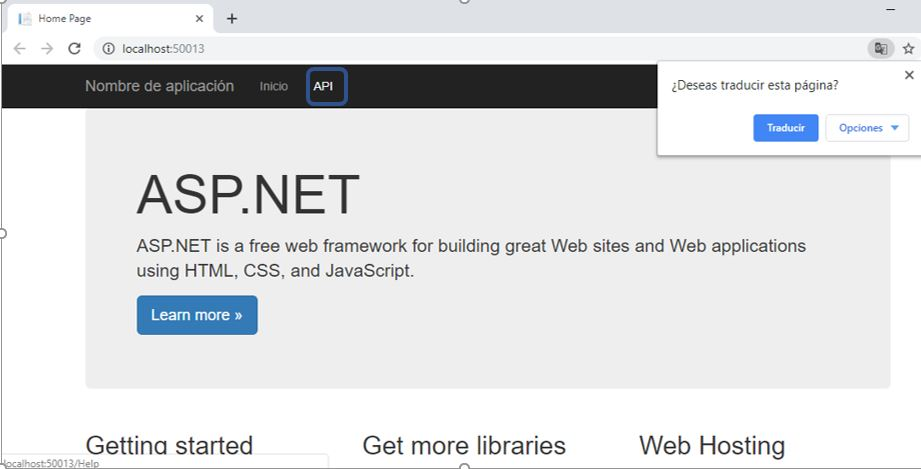
\includegraphics[width=15cm]{./Imagenes/Captura19}
	\end{center}
	\item Paso 18: Nos mandara a otra pagina en la que debemos buscar la opcion	(POST api/Alumnos) y la seleccionamos\\
	\begin{center}
		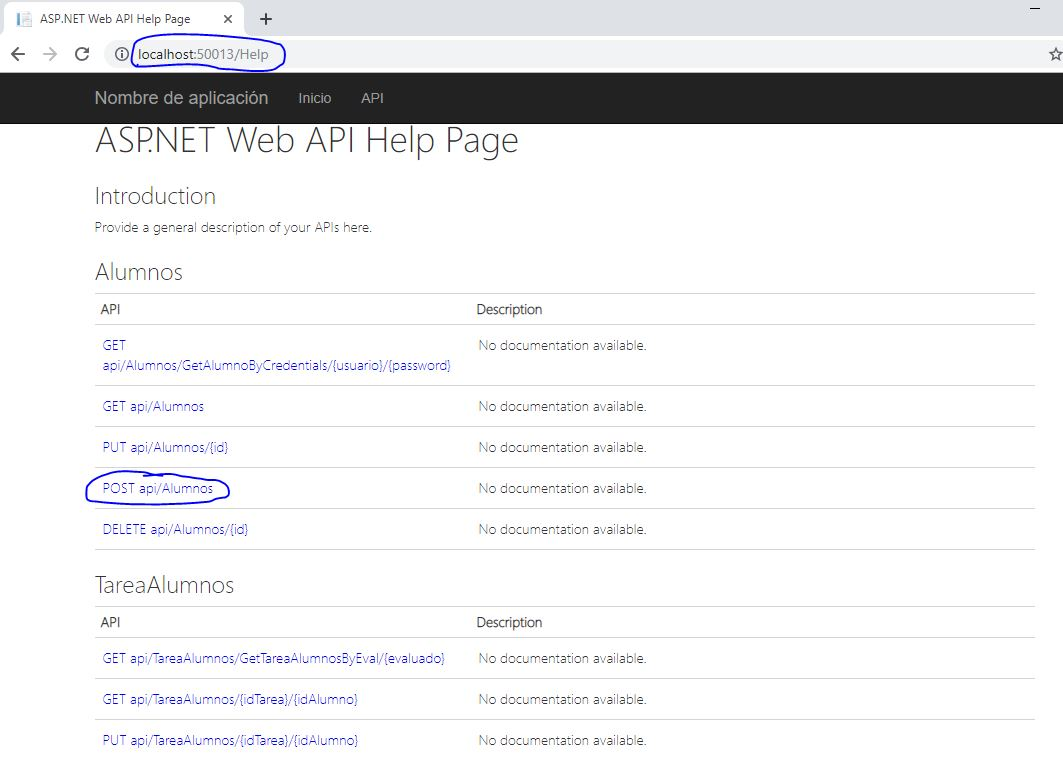
\includegraphics[width=15cm]{./Imagenes/Captura20}
	\end{center}
	\item Paso 19: Ahora hay que buscar un bloque de texto que se llame(application/json, text/json)\\
	Copiamos el ejemplo\\
	\begin{center}
		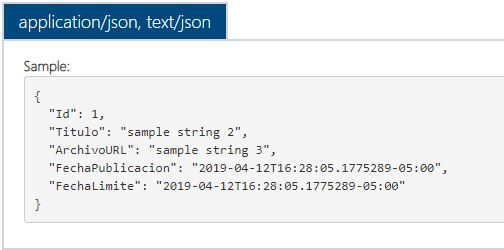
\includegraphics[width=15cm]{./Imagenes/Captura21}
	\end{center}
	\newpage
	\item Paso 20: Descargamos Postman, y lo instalamos, para luego dentro de postman abrimos una pestaña nueva dentro del mismo y hacemos lo siguiente\\
	\begin{center}
		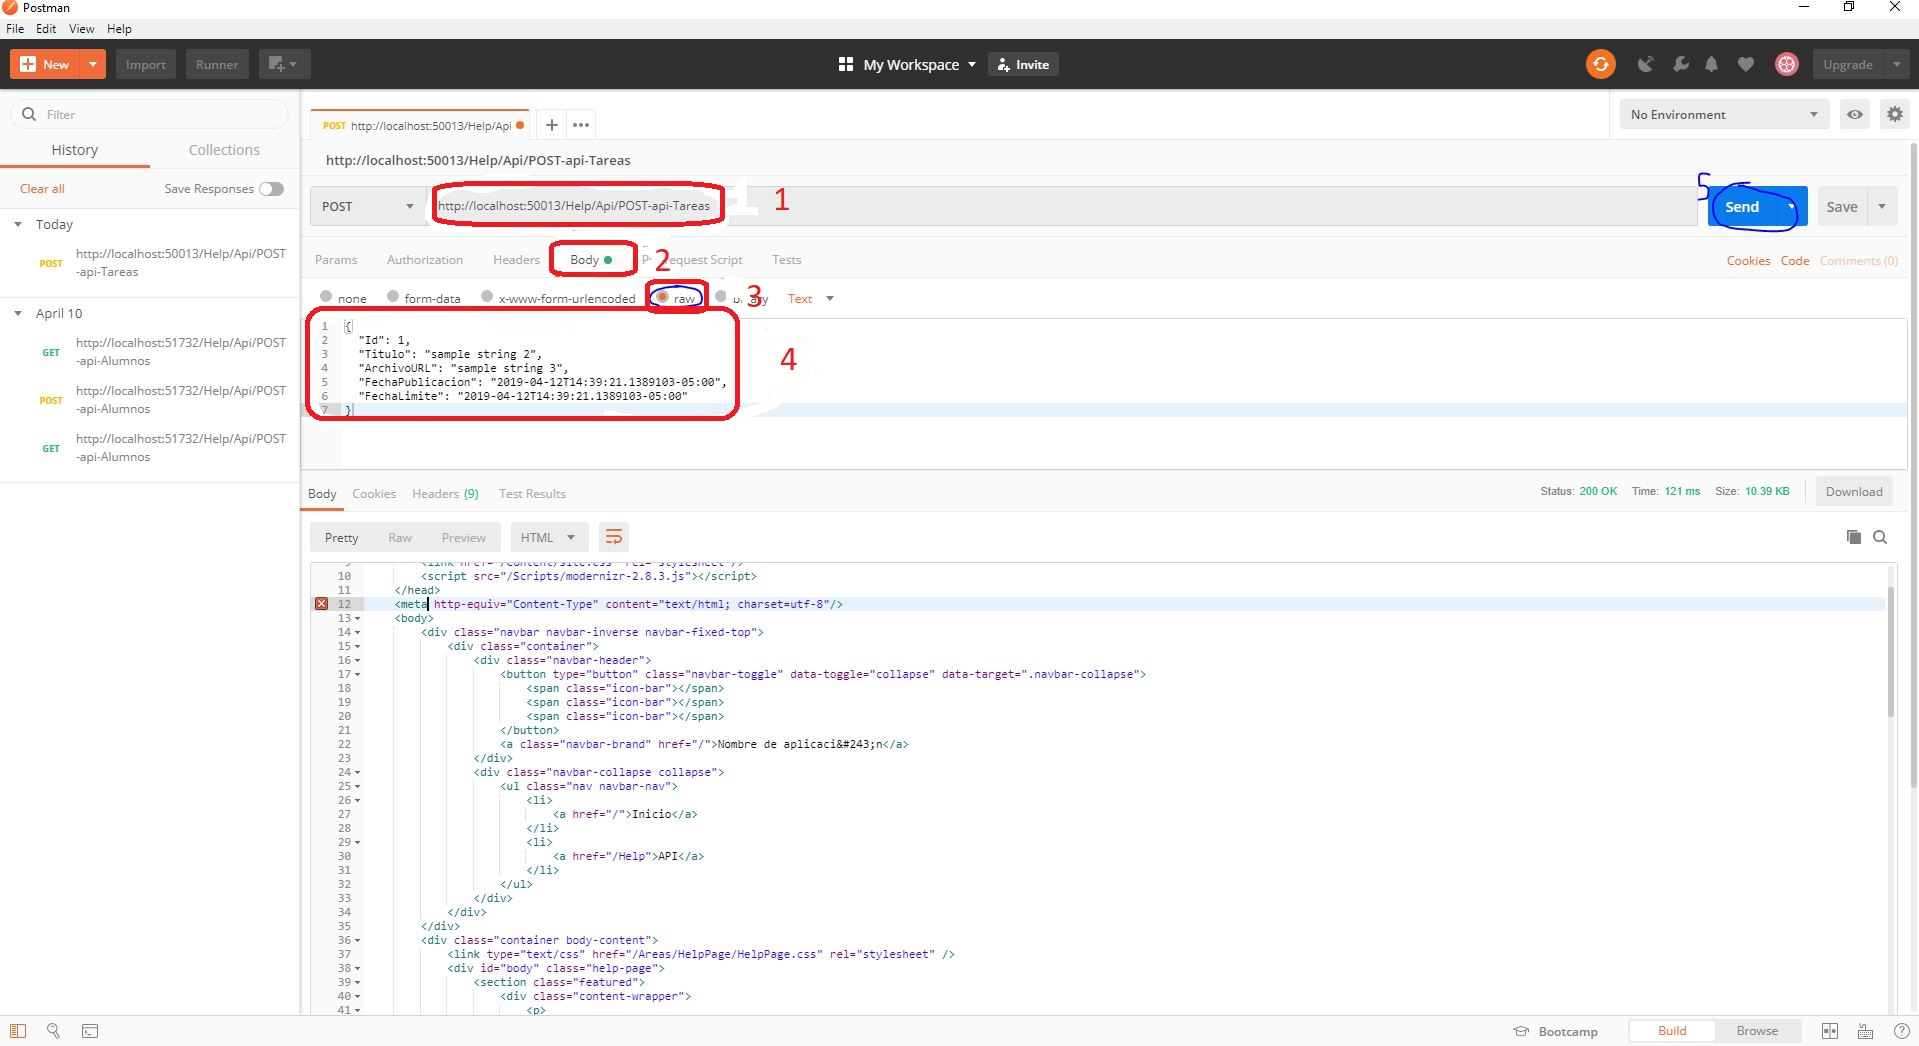
\includegraphics[width=15cm]{./Imagenes/Captura22}
	\end{center}
	
	
	
\end{itemize}





